\documentclass[10pt,a4paper,notitlepage]{article}
\usepackage[utf8]{inputenc}
\usepackage{amsmath}
\usepackage{amsfonts}
\usepackage{amssymb}
\usepackage{bm}
\usepackage{fullpage}
\usepackage{lastpage}
\usepackage{lscape}
\usepackage{fancyhdr}
\usepackage{multirow}
\usepackage{fancyvrb}
\usepackage{xcolor}
\usepackage{tikz}
\usepackage{graphicx}
\graphicspath{{./Graphics/}}
\usepackage{float}
\usepackage{nameref}
\usepackage{parskip}
\usepackage{setspace}

\usepackage[backend=bibtex,style=alphabetic]{biblatex}
\addbibresource{References.bib}
  
\author{Jonah M. Gibbon}

\pagestyle{fancy}
\fancyhf{}
\renewcommand{\headrulewidth}{0pt}
\cfoot{Page \thepage\ of \pageref{LastPage}}

\newif\ifsubmission

\newcommand{\abs}[1]{\lvert#1\rvert}
\newcommand{\Z}{\mathbb{Z}}
\newcommand{\Q}{\mathbb{Q}}
\newcommand{\C}{\mathbb{C}}
\newcommand{\N}{\mathbb{N}}
\newcommand{\R}{\mathbb{R}}
\newcommand{\Prob}{\mathbb{P}}
\newcommand{\E}{\mathbb{E}}
\newcommand{\Pois}{\text{Pois}}
\newcommand{\x}{\textbf{x}}
\newcommand{\iid}{\stackrel{\text{iid}}{\sim}}

\newcommand{\candidatenumber}{1234N}
\newcommand{\college}{Girton College}
\newcommand{\course}{Mathematics Tripos, Part III}

\newtheorem{theorem}{Theorem}


\renewcommand{\refname}{Reference}

\title{\Huge Measuring the Unmeasurable \\ \vspace{0.4cm}  \huge Part III Essay}

\begin{document}
\begin{titlepage}
\makeatletter

% University logo with shield hanging in left margin

\includegraphics[width=75mm]{ucam-logo-bw}

\begin{center}
\huge
\vspace{\fill}

\@title
\vspace{\fill}



\end{center}


\vspace{\fill}
\begin{center}
Submitted in fulfillment of the requirements for the\\
\course
\end{center}

\makeatother
\end{titlepage}


\begin{center}
With thanks to Tina Marjanov at the Computer Laboratory, \\Cambridge for their technical help.
\end{center}
\tableofcontents
\pagebreak
\section{Introduction}
Estimating the unknown size of a population $N$ is a familiar problem and has many possible approaches; the simplest and most widely understood being the capture-recapture method. It was originally presented by Sekar \textit{et al} in \cite{Sekar} in the 1940s where it was first used to estimate the size of a human population.  It is outlined as follows: suppose that $A_{1}$ and $A_{2}$ denote uniform samples with replacement from a population (the size of the samples may be random). An estimate for the size of the total population is then given by
\begin{equation}
\hat{N}=\frac{\abs{A_{1}}\cdot \abs{A_{2}}}{\abs{A_{1}\cap A_{2}}}
\end{equation}
where $\abs{S}$ denotes the size of set $S$. In the same paper an estimate for the variance of $\hat{N}$ is derived:
\begin{equation}
\text{Var}\left(\hat{N}\right)=\frac{\abs{A_{1}}\cdot\abs{A_{2}}\cdot\abs{A_{1}\backslash A_{2}}\cdot\abs{A_{2}\backslash A_{1}}}{\abs{A_{1}\cap A_{2}}^{3}}
\end{equation}
As described by Sekar, the estimate $\hat{N}$ relies on the assumptions that the two samples are drawn independently,  all members in the population having an equal chance of being sampled, and $\abs{A_{i}}$ are sufficiently large (this estimator holds asymptotically). These impose tight assumptions on the population, making this estimate difficult to work with in practice. 

When using this method to estimate criminal activity, all of these assumptions don't hold, and as a result the estimate is not helpful. The population of criminals is believed to be largely undetected, and as a result sample sizes are small, violating the asymptotic condition, as well as $\abs{A_{1}\cap A_{2}}$ being small leading to a large variance in the final estimate. Criminal offences are not drawn uniformly from the criminal population, as it's not unreasonable to believe re-offenders are more likely to get caught. This is because they have already been processed by the authorities and are likely to be under closer supervision. Finally sentences for re-offenders tend to be higher, and so it is reasonable to believe criminals are less likely to re-offend given they have already been caught.  This means the samples $A_{1}$ and $A_{2}$ are not independent.\footnote{For serious crimes (ones that carry prison sentences), the criminal population may have changed over the period of their sentence, and hence the samples $A_{1}$ and $A_{2}$ are not independent, conditional on them re-offending after they are released. }

This essay will concern itself with estimating the size of hidden populations, defined for our purposes as a group of people that for some inherent reason wish to remain hidden, such as criminal groups. Due to this concealed activity many of the assumptions required for the capture-recapture method don't hold, such as the example above, and a new approach must be taken. In the paper \cite{Silverman} by Silverman several new methods are defined, motivated by the data collected by the National Crime Agency regarding potential victims of human trafficking in the UK, 2013 (see Silverman, \cite{Silver}). One of these methods will be analysed in detail later in this essay, as well as being compared to the others.



The data that will be analysed in this essay will be a collection of online extremist posts across different forums between 2018 and 2021 collected by the Computer Laboratory in Cambridge. Although this data is not publicly available, an analysis of it can be found in the paper \cite{ExtremeBB} by Anh V. Vu \textit{et al}. This data will be introduced in more detail later. 

An overview of this essay is as follows. In section \ref{sc:2} the online dataset is introduced in more detail, and the classification of the data is reviewed. In section \ref{sc:3} a probabilistic model for the population $N$ given theoretical data $\mathcal{N}$ is introduced. This is expanded on in section \ref{sc:4} where a Markov Chain Monte Carlo (MCMC) algorithm to estimate the distribution $P(N\mid\mathcal{N})$ is presented. In section \ref{sc:5} Silverman's other approaches are compared to the MCMC method, with reasons why they have not been used for the online dataset. The results from applying the MCMC algorithm to the online data set are presented in section \ref{sc:6} along with a short conclusion discussing further research.

The main approach to estimate $N$ discussed in this essay is drawn from the paper \cite{BayesianMixing} by Daniel Manrique-Vallier. All code written to produce the results in this essay is original and referenced in the GitHub repository \cite{Jonah}, along with a collection of datasets used throughout. The appropriate code will be referenced as necessary throughout the essay. 

All data in this essay will be multiple systems data, and all methods discussed are forms of multiple system estimation (MSE). This means the data has been collected across multiple sources before being integrated together such that common data is not over counted. A more detailed explanation of multiple systems data can be found in the papers \cite{Systems} by Samuelsen \textit{et al}, and \cite{Silver} by Silverman. It is important to note that the vast majority of data is not of this form, and as a result the MSE methods discussed in this essay do not apply in general.
\section{The Data Sets}\label{sc:2}
In this section, the main dataset that will motivate the essay is introduced. The original classification of this data will be reviewed, as well as introducing simulated data and the human trafficking data from \cite{Silver} to test the accuracy of the methods in this essay. The simulated data and human trafficking data are available in the GitHub repository \cite{Jonah}, however due to Cambridge University regulations, the online data has not been made publicly available. I would like to thank Tina Marjanov from the Computer Laboratory for her technical help accessing this online data.
\subsection{ExtremeBB}
\subsubsection*{Introduction}
\texttt{ExtremeBB} is an actively maintained database comprising of 45 million radical comments made online across 19 public forums based in America. As well as the comments themselves, usernames and timestamps of each post, some dating as far back as 2001, have been collected to better understand how these online extremists interact. Each forum has a common theme such as white supremacy, making cross forum analysis an interesting topic of research, as it investigates the overlap between these radical beliefs. This essay focuses on the overlap of usernames across different forums, to give an improved estimate for the number of active online extremists in America, and how that number has changed between 2018 and 2021. For more information about the dataset, see the paper \cite{ExtremeBB} by Anh V Vu \textit{et al}.

To apply MSE we must classify users that lie in multiple forums, however there is no gold standard method in doing this. Users that are active on multiple sites aren't required to use the same usernames, and as a result it is difficult to confidently classify two usernames as the same person. However, there are ways to approach this problem, such as comparing when users regularly post and searching for similar usernames that are likely to be the same person.

This problem was investigated in Anh's paper, where two usernames were classified as the same person if three conditions were fulfilled:

First the two usernames had to match identically. 

Secondly the matched username must be classified as 'rare' since usernames like \texttt{Glory} are likely to be used by two or more users by chance (see the paper \cite{27} by Lui \textit{et al}). Determining if a username is 'rare' is done by segmenting each username into a word sequence, and then it's n-gram probability metric is estimated by a language model trained on the data 'Reuters corpus' (see the paper \cite{gram} by Lui \textit{et al} for the model, and the paper \cite{corpus} by Russel-Rose \textit{et al} for the training data).\footnote{The details of how a username is deemed rare has been deliberately left out, as it does not contribute to this essay. More details can be found in the appropriate references.} This metric was required to be less than 1\%.

Finally users had to post at approximately the same time of day to be deemed as the same user. This was done by calculating each username's posting distribution $P_{u}$, a discrete probability distribution taking values on $\{0,1,\hdots, 23\}$ defined as
\begin{equation}
P_{u}(i)=\frac{\text{Number of posts made by username } u \text{ between the hours }i \text{ and } i+1}{\text{Total number of posts made by username }u}
\end{equation}
For brevity let $P_{i}$ denote the posting distribution of username $u_{i}$. This gives an approximate distribution of when each username would post. To classify if two usernames $u_{i},u_{j}$ had similar posting distributions, the quantity $(D(P_{i}||P_{j})+D(P_{j}||P_{i}))/2$ was required to be less than 1, where $D(P_{i}||P_{j})$ denotes the Kullback-Leibler divergence defined as
\begin{equation}
D(P_{i}||P_{j})=\sum_{k=0}^{23}P_{i}(k)\log_{2}\left(\frac{P_{i}(k)}{P_{j}(k)}\right)
\end{equation}

This criterion developed by Anh helps to provide better estimates for the number of users spanning multiple forums, however it is flawed. Specifying that the usernames are identical does not account for those using different handles, and hence underestimates the overlap between forums. Using the Kullback-Leibler divergence to measure the similarity between posting distributions is a volatile choice, as it easily diverges to infinity (when $P_{j}(k)=0$ and $P_{i}(k)\neq 0$ for some $i,j,k$). Furthermore, many of the posting distributions within \texttt{ExtremeBB} are sporadic and small, with some users only posting once or twice, causing this phenomenon to frequently occur. This is why I propose a new classification criterion, and argue why it is improved.

\subsubsection*{Classification Alterations}
Firstly, the condition that usernames must match exactly can be relaxed, to instead matching them approximately. Behavioural studies (see the paper \cite{Sites}) show different usernames used by the same person are more likely to be 'similar', such as \texttt{John} and \texttt{John1}. To match these similar usernames, we introduce the Levenshtein distance. It is a string metric that measures the similarity between two strings $a$ and $b$. It is defined as the minimum number of single character edits (insertions, deletions or substitutions) needed to transform $a$ into $b$, and is denoted by $\text{lev}(a,b)$. For example, $\text{lev}(\texttt{kitten},\texttt{sitting})$ has a distance of 3, since we can transform $\texttt{kitten}\rightarrow\texttt{sitten}\rightarrow\texttt{sittin}\rightarrow\texttt{sitting}$.

Calculating the the Levenshtein distance between strings $a$ and $b$ can be done in $O(\abs{a}\cdot\abs{b})$ order operations, where $\abs{a}$ denotes the string length of $a$ (see the Wagner–Fischer algorithm presented in the paper \cite{Fisher} by Wagner and Fisher). Due to the size of \texttt{ExtremeBB} quadratic complexity is not fast enough, and so for our purposes we classify two usernames as the same user if they have a distance of 1 or less. This property can be calculated in a linear number of operations, as exploits the property that if two usernames differ in length by two or more, then so does the Levenshtein distance. For more information on how this is achieved, see the function \texttt{Fuzzy} defined in the code \texttt{Data-Classier} in the GitHub repository. 

Secondly, I propose using a different divergence than the Kullback-Leibler to compare the posting distributions of different usernames. Since we anticipate data lying in the intersections of more than two forums, a divergence that generalises to more than two distributions would be beneficial, as well as one that is bounded to computationally compare the small and sporadic distributions in \texttt{ExtremeBB}. I propose using the Jenson-Shannon divergence (JSD), defined as
\begin{equation}
\text{JSD}(P_{1},\hdots,P_{n})=H\left(\frac{1}{n}\sum_{i=1}^{n}P_{i}\right)-\frac{1}{n}\sum_{i=1}^{n}H(P_{i})
\end{equation}
where $H(P)$ denotes the entropy of the distribution $P$, defined as
\begin{equation}
H(P)=-\sum_{i=0}^{23}P(i)\log_{2}\left(P(i)\right)
\end{equation}
This divergence fulfils both requirements; that it generalises to more than two distributions and is bounded, with $\text{JSD}(P_{1},\hdots,P_{n})\leq \log_{2}(n)$ (see the paper \cite{Shan} by Lin for a proof).

Calculating the JSD for each combination of posting distributions is computationally strenuous as it involves calculating the JSD $O(2^{U})$ times, where $U$ is the total number of different usernames. However, by imposing that pairwise distributions are 'close', that is the $\text{JSD}(P_{i},P_{i+1})\leq\varepsilon$ for all $i=1,\hdots,U$, where $P_{U+1}=P_{1}$ and $\varepsilon >0$, then we can deduce that larger combinations of distributions are also 'close', and hence do not need to be checked. 

Starting with the above assumption and the inequality $H(X_{1}+X_{2}+X_{3})+H(X_{2})\leq H(X_{1}+X_{2})+H(X_{2}+X_{3})$ for arbitrary discrete distributions $X_{i}$ (brief proof in Madiman, \cite{madiman2008entropy}) the following can be derived:
\begin{equation}
\begin{aligned}
H\left(\sum_{i=1}^{n}\frac{1}{n}P_{i}\right) &\leq \sum_{i=1}^{n-1}H\left(\frac{1}{2}P_{i}+\frac{1}{2}P_{i+1}\right)-H\left(P_{i+1}\right)+H(P_{n})\\
&\leq (n-1)\varepsilon +\frac{1}{2}H(P_{1})+\frac{1}{2}H(P_{n})
\end{aligned}
\end{equation}
Since the $P_{i}$ can be arbitrarily switched in the sum, the following can be concluded:
\begin{equation}
\text{JSD}(P_{1},\hdots,P_{n})\leq (n-1)\varepsilon
\end{equation}
Therefore by bounding pairwise distributions, which involves calculating the JSD $U$ times, we can impose a bound on all combinations of greater than two distributions. Although this bound grows quicker in $n$ than the one guaranteed by $\log_{2}(n)$, if we assume that no user is active on $n$ or more forums and choose $\varepsilon < \log_{2}(n-1)/(n-2)$ we impose a tighter restriction on the posting distributions.

Finally in Anh's paper there was no analysis of how the overlap of users have evolved over time. Since \texttt{ExtremeBB} is a large database, I've broken down the data into 3 month time periods to better understand this trend. Because of this, I decided to relax the 'rarity' condition, since the data spans a much shorter time frame, and so the chances of falsely comparing two common usernames is considerably less than in the original analysis \cite{ExtremeBB}. This is why the specifics of this criterion have been deliberately left out. 

These three conditions form my modified classification conditions.
\subsubsection*{Summary of Data}
The classification of these usernames was done over nine different forums\footnote{These forums are summarised as follows: SF - Stormfront, IS - Incelsis, IN - Incelsnet, LS - Lookism, RV - RooshV, PA - Pickup Artistry, MW - Men Going Their Own Way, GW - Going Your Own Way, KF - Kiwifarms.}, since many of the original 19 were not old enough or active enough to produce valid time-sequential conclusions. Initially only the fuzzy matching condition was used to classify the data to find an upper bound on the greatest number of forums a user would span. This ended up equalling 3, and so $\varepsilon$ was chosen to equal $3/4<\log_{2}(3)/2$ to restrict how 'close' pairwise posting distributions should be. A portion of classified data detailing the activity of users between the 1st Jan 2020 and the 31st March 2020, produced by the code \texttt{Data-Classifier}, is tabulated below in Table \ref{tb:1}. Here the first 9 columns denote which intersection of forums each case lies in, with the symbol $\times$ denoting if the user was active in that forum and left blank if they weren't, and the count data in the tenth column.  Combinations of forums that had no active users have been omitted from the table. Due to the size of the data, only a portion of it is presented. For example there were 2 users that were active only on forums Incelsnet, RooshV and Kiwifarms, whose usernames and posting distributions passed the modified classification conditions. 

An interesting observation is that despite the relaxed classification conditions, the size of the intersections between forums is much less than that published in Anh's paper. This suggests that many of the users were active over a long period of time, and changed forums irregularly.

This data will be revisited in section 6 when discussing estimates for the number of active online extremists.

\begin{table}[H]
\centering
\begin{tabular}{|ccccccccc|c|}
\hline SF & IS & IN & LS & RV & PA & MW & GW & KF & Count \\ \hline
$\times$&&&&&&&&& 1543\\
&$\times$&&&&&&&& 1418\\
&&$\times$&&&&&&& 736\\
&&&$\times$&&&&&& 1793\\
&&&&$\times$&&&&& 858\\
&&&&&$\times$&&&& 2\\
&&&&&&$\times$&&& 125\\
&&&&&&&$\times$&& 82\\
&&&&&&&&$\times$& 8032\\ \hline
$\times$&$\times$&&&&&&&& 1\\
$\times$&&$\times$&&&&&&& 1\\
$\times$&&&$\times$&&&&&& 2\\
$\times$&&&&$\times$&&&&& 1\\
$\times$&&&&&$\times$&&&& 1\\
$\times$&&&&&&$\times$&&& 2\\ 
$\vdots$&$\vdots$&$\vdots$&$\vdots$&$\vdots$&$\vdots$&$\vdots$&$\vdots$&$\vdots$&$\vdots$\\
&&$\times$&$\times$&&&&&$\times$&1\\
&&&$\times$&$\times$&&&&$\times$ &2\\
&&&&$\times$&&&$\times$&$\times$&1\\ \hline
&&&&&&&&Total&14724\\ \hline
\end{tabular}
\caption{Portion of data on the number of active extremist users between 01/01/2020 and 31/03/2020 matched across combinations of forums using the modified classification conditions and data from \texttt{ExtremeBB}}\label{tb:1}
\end{table}
\subsection{Human Trafficking Data}
In order to compare how Silverman's original methods compare to the one developed in this essay, we introduce the human trafficking data \texttt{HumanTrafficking} presented in \cite{Silver}. It is tabulated in Table \ref{tb:3} below, formatted in the same way as in Table \ref{tb:1}. Note the headings in Table \ref{tb:3} denote different authorities that were involved with each case, although in this essay it is not important to specify them. 

One of the main differences between \texttt{ExtremeBB} and \texttt{HumanTrafficking} is the number of lists that the data falls into, respectively 9 and 5. Silverman relied heavily on methods that exploited a small number of lists (at most 5), and at times was forced to edit the data for these methods to work. This is what has been done in column three, as described by Silverman in his paper. When processing \texttt{ExtremeBB}, we must develop a method that scales computationally with the number of lists the data falls into.

Another notable difference is the number of observed cases, with \texttt{ExtremeBB} having over 5 times as many cases as \texttt{HumanTrafficking}. This will lead to a computational strain when processing the online data, as seen in section \ref{sc:4}.

We will not return to this data until section \ref{sc:5} when using it to compare Silverman's proposed methods.
\begin{table}[H]
\centering
\begin{tabular}{|ccccc|c|}
\hline LA & NG & PF+NCA & GO & GP & Count \\ \hline
$\times$&&&&& 54\\
&$\times$&&&& 463\\
&&$\times$&&& 933\\
&&&$\times$&& 695\\
&&&&$\times$& 316\\ \hline
$\times$&$\times$&&&& 15\\
$\times$&&$\times$&&& 19\\
$\times$&&&$\times$&& 3\\
&$\times$&$\times$&&& 62\\
&$\times$&&$\times$&& 19\\
&$\times$&&&$\times$& 1\\
&&$\times$&$\times$&& 76\\
&&$\times$&&$\times$& 11\\
&&&$\times$&$\times$& 8\\ \hline
$\times$&$\times$&$\times$&&& 1\\
$\times$&$\times$&&$\times$&& 1\\
&$\times$&$\times$&$\times$&& 4\\ \hline
$\times$&$\times$&$\times$&$\times$&& 1\\ \hline
&&&&Total&2744\\ \hline
\end{tabular}
\caption{Potential victims of trafficking in the UK, 2013: numbers of cases on each possible combination of lists}\label{tb:3}
\end{table}

\subsection{Simulated Data}
In order to confirm that the method developed in this essay is accurate with a large number of lists, a simulated data set \texttt{TestData} was generated under the conditions in section \ref{sc:3} using the code \texttt{Simulated-Data}. This data was intended to imitate \texttt{ExtremeBB} in the closest possible way, and hence the number of lists was set to $9$. The true population size was set to $N=1000$, and the probability that a case lay in the intersection of $m$ lists was proportional to an i.i.d (independent and identically distributed) $\text{Gamma}(3/(m+1),1)$ variable. This was to create the effect of a sparse data set where not many individuals lay in the intersection of many lists. Finally the data was generated under a multinomial model and the 'unobserved cases' ($m=0$) were removed, as described further in section \ref{sc:3}. This data will be revisited at the end of section 4, where after establishing the method of estimating the size of the population, the plausibility of the method is discussed.

\section{Model Assumptions}\label{sc:3}
In this section the theoretical framework for a Bayesian analysis to estimate the unknown population size $N$ is developed. This approach is motivated by that of Daniel Manrique-Vallier in \cite{BayesianMixing}, and will be further built on in section \ref{sc:4}.
\subsection{Notation}
Before introducing the model for estimating the size of the unknown population, it is important to introduce some notation. Let the set of lists be denoted $L=\{1,\hdots,K\}$, and the power set of $L$ as $\mathcal{P}(L)$. Let $n_{S}$ denote the number of cases that appear in $S\in\mathcal{P}(L)$ and not in $\mathcal{P}(L)\backslash S$. For example, using the data in Table \ref{tb:1}, $n_{\{1,3\}}=2$. Notice it is sufficient to estimate $n_{\emptyset}$, the number of unobserved cases, since $N=n+n_{\emptyset}$, where $n:=\sum_{\emptyset \neq S\in \mathcal{P}(L)}n_{S}$ is the total number of observed cases.

Let $\left(\x_{i}\right)_{i=1}^{N}$ denote which intersection each individual case lies in. This is done by denoting $\x_{i}\in\{0,1\}^{K}$, where $(\x_{i})_{j}=1$ if observation $\x_{i}$ is present in list $j$, and 0 otherwise. Notice there is the natural bijection between $\{0,1\}^{K}$ and $\mathcal{P}(L)$, and hence the abuse of notation $\x_{i}=S$ will be used to denote $(\x_{i})_{j}=1\iff j\in S$. Using this notation, the identity $n_{S}=\sum_{i=1}^{N}\mathbf{1}(\x_{i}=S)$ is recovered.

\subsection{Multinomial Model}\label{sc:3.2}
\subsubsection*{Overview}
Here, the main model that will be used in this essay is introduced: the multinomial model. Suppose $N$ was a fixed yet unknown quantity, and each individual case fell randomly into the intersection of each list with probability $f(\x\mid\theta)$, where $\theta$ is some shape parameter. Then the probability of observing the data $\mathcal{N}=(n_S)_{\emptyset\neq S\in\mathcal{P}(L)}$ would be the multinomial model
\begin{equation}\label{eq:Multinomial}
P\left(\mathcal{N}\mid\theta,N\right)=\frac{N!}{(N-n)!} \cdot f(\mathbf{0}\mid\theta)^{N-n}\prod_{\substack{\emptyset\neq S\in\mathcal{P}(L)\\ \x=S}}\left\lbrace \frac{f(\x\mid \theta)^{n_{S}}}{n_{S}!}\right\rbrace\mathbf{1}(N\geq n)
\end{equation}
Therefore it suffices to specify $f(\x\mid\theta)$ to fully determine the model. 

In the rare case where the lists can be deemed independent, in other words the probability of lying in list $i$ is independent of the probability of lying in list $j$ for all $i,j$, then the natural model to be chosen would be the product-Bernoulli distribution
\begin{equation}
f(\x\mid\bm{\theta})=\prod_{i=1}^{K}(\theta_{i})^{x_{i}}(1-\theta_{i})^{1-x_{i}}
\end{equation}
where $\theta_{i}$ denotes the probability of lying in list $i$, and $x_{i}=(\x)_{i}$. However this is a restrictive model, and one that is unlikely to be true in practice. Certainly with the data in \texttt{ExtremeBB}, it's not unreasonable to assume that members are more likely to be active on forums that share common themes, for instance, both RooshV and Pickup Artistry, since these are two forums that have similar topics of conversation.  As a result, a more flexible model for $f(\x\mid\theta)$ is required.

\subsubsection*{The Latent Class Model}
To address this problem, a Latent Class Model (LCM) can be applied. This is defined as a mixture of independent product-Bernoulli distributions. The concept involves finding $M$ substrata of the population such that an independent product-Bernoulli distribution is valid, conditional on the case lying in this substrata. This involves introducing a latent random variable $z\sim\text{Discrete}(\{1,\hdots,M\})$ to assign each observed case to a substrata.
Formally, this mixture model is defined as
\begin{equation}
f(\x\mid\bm{\theta})=\sum_{m=1}^{M}\left\lbrace\pi_{m}\prod_{i=1}^{K}(\theta_{im})^{x_{i}}(1-\theta_{im})^{1-x_{i}}\right\rbrace
\end{equation}
where $\pi_{m}=\Prob(z=m)$ denotes the probability of lying in substrata $m$. This model places no assumptions on $f(\x\mid\theta)$, as it's proved by Dunson and Xing in \cite{BinomialMixingGood} that any discrete distribution on $\{0,1\}^{K}$ can be represented by a mixture of product-Bernoulli distributions. \\

A brief outline of the proof is as follows. Let 
\begin{equation}
\bm{\pi}=\{\Prob(\x_{1}=c_{1},\hdots,\x_{K}=c_{K}) : c_{i}\in\{0,1\} \,\, \forall \,\,1\leq i\leq K\}\in\Pi_{K}
\end{equation}
where $\bm{\pi}$ denotes a higher order tensor, with $\Pi_{K}$ denoting all discrete probability tensors on $\{0,1\}^{K}$. Probability tensors have non-negative elements and $\abs{\abs{\bm{\pi}}}_{1}=1$. Using a singular value decomposition of the tensor, $\bm{\pi}$ may be represented as
\begin{equation}
\bm{\pi}=\sum_{i=1}^{M}\alpha_{i}\mathbf{U}_{i} \quad \quad\quad\quad\quad\quad \mathbf{U}_{i}=\mathbf{u}_{i}^{(1)}\otimes\mathbf{u}_{i}^{(2)}\otimes\hdots\otimes\mathbf{u}_{i}^{(K)}
\end{equation}
where $\alpha_{1}\geq\hdots\geq\alpha_{M}>0$, $\mathbf{U}_{i}$ is a decomposed tensor, and $\mathbf{u}_{i}^{(j)}\in\R^{2}$, $M\in\N$. By rescaling, $\alpha_{i}$ forms a probability distribution and each $\mathbf{u}_{i}^{(j)}$ forms a probability vector. This is the result required.

\subsubsection*{The Non Parametric Latent Class Model}
Although the LCM is a useful step towards specifying the model in equation \eqref{eq:Multinomial}, it does introduce the problem of calculating the size of $M$ and which substrata these product-Bernoulli distributions are valid on. In the same paper \cite{BinomialMixingGood}, Dunson and Xing propose a Bayesian non parametric extension of the LCM, called the Non Parametric Latent Class Model (NPLCM). This involves letting the number of substrata $M$ tend to infinity, while simultaneously choosing priors that induce sparsity into the model by concentrating the probability into the first few substrata. The benefit of this method is that it removes unnecessary specification of the value of $M$, as well as creating a sparse model for analysis.

Formally, the NPLCM can be defined through the hierarchical process:
\begin{align*}
x_{i} \mid z &\sim \text{Bernoulli}(\theta_{iz})  & &1\leq i\leq K\\
z &\sim \text{Discrete}(\N,(\pi_{1},\pi_{2}, \hdots)) & &\\
\bm{\theta}:= \theta_{i,j} &\iid \text{Beta}(1,1) & &1\leq i\leq K, j\in\N\\
\bm{\pi} := (\pi_{1},\pi_{2},\hdots ) &\sim \text{SB}(\alpha) &&\\
\alpha &\sim \text{Gamma}(a,b) &&\\
\end{align*}
where SB$(\alpha)$ denotes the 'Stick Breaking Process'.

The stick breaking process is a Dirichlet process used to draw a random infinite-discrete distribution of decreasing probabilities, such that there is sparsity away from the first few probabilities. The process is simple: for each $i\geq 1$, take $\beta_{i}\iid\text{Beta}(1,\alpha)$ and set $\pi_{i}=\beta_{i}\prod_{j=1}^{i-1}(1-\beta_{j})$. This is equivalent to taking a $\text{Beta}(1,\alpha)$ random position on a unit length stick, and marking this position as $\pi_{1}$. Then discarding the stick to the left of $\pi_{1}$, mark an iid position on what's to the right of $\pi_{1}$ and call this $\pi_{1}+\pi_{2}$. By repeating this, an infinite random sequence of positive numbers is formed such that they sum to 1, as well as having the majority of their probabilities concentrated in the first few terms. Notice the smaller the value of $\alpha$, the greater $\beta_{i}$ will be on average, and thus the quicker $\pi_{i}$ will converge to zero (almost surely) and the more concentrated the resultant distribution will be in the first few terms. 

Returning to equation \eqref{eq:Multinomial}, the complete conditional model for $P(\mathcal{N}\mid\bm{\theta},\bm{\pi}, N)$ is 
\begin{equation}
\frac{N!}{(N-n)!}\left\lbrace \sum_{m=1}^{\infty}\pi_{m}\prod_{i=1}^{K}(1-\theta_{im})\right\rbrace^{N-n}\prod_{\substack{\emptyset\neq S\in\mathcal{P}(L)\\ \x=S}} \frac{1}{n_{S}!}\left\lbrace\sum_{m=1}^{\infty}\pi_{m}\left\lbrace\prod_{i=1}^{K}\left(\theta_{im}\right)^{x_{i}}\left(1-\theta_{im}\right)^{(1-x_{i})}\right\rbrace\right\rbrace^{n_{S}}
\end{equation}
multiplied by the indicator function $\mathbf{1}(N\geq n)$. Although this answer is correct, it is difficult to work with, and rewriting it using the latent variable $\mathbf{z}$ makes it easier for Bayesian analysis. Note the above is equivalent to marginalising $P(\mathcal{N},\mathbf{z}\mid\bm{\theta},\bm{\pi},N)$ over $\mathbf{z}$, where $P(\mathcal{N},\mathbf{z}\mid\bm{\theta},\bm{\pi},N)$ is defined as
\begin{equation}\label{eq:Final}
\frac{N!}{(N-n)!}\prod_{i=1}^{N-n}\pi_{z^{\emptyset}_{i}}\prod_{j=1}^{K}(1-\theta_{jz^{\emptyset}_{i}})\times\prod_{\substack{\emptyset\neq S\in\mathcal{P}(L)\\ \x=S}}\left\lbrace\frac{1}{n_{S}!}\prod_{i=1}^{n_{S}}\pi_{z^{S}_{i}}\prod_{j=1}^{K}(\theta_{jz^{S}_{i}})^{x_{j}}(1-\theta_{jz^{S}_{i}})^{(1-x_{j})}\right\rbrace
\end{equation}
multiplied by $\mathbf{1}(N\geq n)$. Here, $\mathbf{z}=\{z^{S}_{i}:S\in\mathcal{P}(L), 1\leq i\leq n_{S}\}$ and each $z^{S}_{i}$ takes values on $\N$.  
This final model is a robust conclusion, as it imposes no assumptions on the distribution of $f(\x\mid\theta)$, as well as being in the appropriate format for Bayesian estimation, as it comprises only of multiplying simple functions together. There will be further discussion later in this essay (section \ref{sc:MCMC}) about ways to sample the posterior distribution, and appropriate priors on $N$.

\section{The Method}\label{sc:4}
In this section the computational limitations of equation \eqref{eq:Final} are highlighted and the appropriate alterations are presented. The conditional distributions of each variable given the others are calculated, as well as outlining a MCMC algorithm to sample from $P(N\mid\mathcal{N})$. This algorithm is tested on the simulated data \texttt{TestData}, before discussing the validity of the method. This section is still motivated by the paper \cite{BayesianMixing} by Daniel Manrique-Vallier.

\subsection{Alterations to the Multinomial Model}\label{sc:4.1}
Sampling from the posterior distribution $P(N\mid\mathcal{N})$ using equation \eqref{eq:Final} can be done using a standard Gibbs Sampler algorithm (GSA); by drawing from the conditional probabilities of each variable given the rest of them. The derivation of the Gibbs Sampler algorithm can be found in \cite{Gib} by Gelfand. To ensure this method works, a few problems must be addressed before outlining the algorithm.

The first problem encountered is computing $\bm{\pi}$, as it is infinite dimensional.  Note that $\pi_{i}$ is sparse and that when $i$ is large enough, the probability of a case appearing in substrata $i$ can be considered negligible. Because of this, $\mathbf{z}$ can be viewed as taking values on the truncated set $\{1,\hdots,M^{*}\}$, where $M^{*}$ is chosen to be sufficiently large. Choosing the exact value of $M^{*}$ will be determined later through means of trial and error. This truncation is achieved by generating $\beta_{i}$ as previously described for $i\leq M^{*}-1$, before setting $\beta_{M^{*}}=1$. This is equivalent to normalising the distribution so that $\sum_{i=1}^{M^{*}}\pi_{i}=1$, since $\sum_{i\leq M}\pi_{i}-1=-\prod_{i\leq M}(1-\beta_{i})$.


The second problem is that the size of $\mathbf{z}$ depends implicitly on $\{z^{\emptyset}_{i} : 1\leq i\leq n_{\emptyset}\}$, and hence implicitly on $N$, and so cannot be conditioned on when using the GSA. To address this, note that $\mathbf{z}^{+} := \{z^{S}_{i}:\emptyset\neq S\in\mathcal{P}(L), 1\leq i\leq n_{S}\}$ can be conditioned on as it places no assumptions on $N$. The remaining variables $\mathbf{z}^{\emptyset}:=\{z^{\emptyset}_{i}:1\leq i\leq n_{\emptyset}\}$ can be replaced with a new set of variables, the number of which do not depend on $N$. This is done by defining $\bm{\omega}\in \N^{M^{*}}$ with $\omega_{k}=\sum_{i=1}^{n_\emptyset}\mathbf{1}(z_{i}^{\emptyset}=k)$, denoting the number of unobserved cases that lie in substrata $k$. The importance of this is it derives a new representation of the model $P(\mathcal{N},\mathbf{z}^{+},\bm{\omega}\mid \bm{\pi},\bm{\theta},N)$ where the number of variables is fixed, namely 
\begin{equation}\label{eq:FINALFINAL}
\begin{aligned}
P(\mathcal{N},\mathbf{z}^{+},\bm{\omega}\mid\bm{\pi},\bm{\theta},N) = &\begin{pmatrix} N\\ n, \omega_{1},\hdots,\omega_{M^{*}}  \end{pmatrix} \prod_{m=1}^{M^{*}}\left(\pi_{m}\prod_{k=1}^{K}(1-\theta_{km})\right)^{\omega_{m}}\\
&\times \prod_{\substack{\emptyset\neq S\in\mathcal{P}(L)\\ \x=S}}\left[\frac{1}{n_{S}!}\prod_{i=1}^{n_{S}}\pi_{z^{S}_{i}}\prod_{j=1}^{K}(\theta_{jz^{S}_{i}})^{x_{j}}(1-\theta_{jz^{S}_{i}})^{(1-x_{j})}\right]\\
&\times \mathbf{1}\left(\sum_{m=1}^{M^{*}}\omega_{m}=N-n\right)
\end{aligned}
\end{equation}
We can exploit the fact that many of the variables are independent of one another, and hence their conditional distributions are standard. In the cases of $\mathbf{z}^{+}$ and $\bm{\theta}$, these are easy to derive and are stated below in section \ref{sc:MCMC}.  However care is needed for the $\bm{\pi}, N$ and $\bm{\omega}$ cases, which are discussed in more detail below.
\subsection{Conditional Probabilities}\label{sc:4.2}
To derive the conditional posterior $P(\bm{\pi}\mid \hdots)$ the stick breaking process must be revisited.\footnote{The $\hdots$ denote all other variables} Previously $\pi_{i}=\beta_{i}\prod_{j=1}^{i-1}(1-\beta_{j})$, where each $\beta_{i}\iid \text{Beta}(1,\alpha)$ for $1\leq i\leq M^{*}-1$. Suppose instead that the $\beta_{i}$ were drawn from independent $\text{Beta}(a_{i},b_{i})$ distributions where the parameters were allowed to change. Connor and Mosimann \cite{Connor} derived that, should the $\beta_{i}$ be chosen in this way, then $P(\bm{\pi}\mid \mathbf{a},\mathbf{b})$ follows a generalized Dirichlet distribution defined as
\begin{equation}
\mathcal{GD}(\x\mid\mathbf{a},\mathbf{b}):= \left[\prod_{i=1}^{M-1}B(a_{i},b_{i})\right]^{-1}x_{M}^{b_{M-1}-1}\prod_{i=1}^{k-1}\left[ x_{i}^{a_{i}-1}\left(\sum_{j=i}^{M}x_{j}\right)^{b_{i-1}-(a_{i}+b_{i})}\right]
\end{equation}
where $\x\in \R^{M-1}$ such that $\x\geq 0$ and $\abs{\abs{\x}}_{1}\leq 1$, $x_{M}:=1-\sum_{i=1}^{M-1}x_{i}$, $B(\cdot,\cdot)$ denotes the Beta function and $(\mathbf{a})_{i}=a_{i}, (\mathbf{b})_{i}=b_{i}$.

It is easy to check that if $a_{i}=1+c_{i}$ and $b_{i}=\beta +\sum_{j=i+1}^{M^{*}}c_{j}$, where $c_{i}$ are constants, then
\begin{equation}\label{eq:GD}
\mathcal{GD}(\x\mid\mathbf{a},\mathbf{b})=\mathcal{GD}(\x\mid \mathbf{\tilde{a}},\mathbf{\tilde{b}})\prod_{i=1}^{M^{*}-1}x_{i}^{c_{i}}
\end{equation} 
where $\tilde{a}_{i}=1$ and $\tilde{b}_{i}=\beta$. This will be a useful result when calculating the conditional probability $P(\bm{\pi}\mid\hdots)$.\\

Since $\sum_{i=1}^{M^{*}}\omega_{i}=n_{\emptyset}$, sampling from the posterior $P(N\mid\hdots)$ is not possible as $\bm{\omega}$ fully specifies $N$. Sampling from the joint conditional distribution $P(N,\bm{\omega}\mid\hdots)$ avoids this problem, which is proportional to 
\begin{equation}
P(N)\frac{N!}{\omega_{1}!\hdots\omega_{M^{*}}!}\rho_{1}^{\omega_{1}}\hdots\rho_{M^{*}}^{\omega_{M^{*}}}\times \mathbf{1}(N=n+n_{\emptyset})
\end{equation}
where $P(N)$ is the prior chosen for $N$, $\rho_{i}:=\pi_{i}\prod_{j=1}^{K}(1-\theta_{ji})$ and $n_{\emptyset}=\sum_{i=1}^{M^{*}}\omega_{i}$. Should $P(N)\propto1/N$ then the above is proportional to
\begin{equation}
\begin{pmatrix} n+n_{\emptyset}-1\\n_{\emptyset}\end{pmatrix} \left(\sum_{i=1}^{M^{*}}\rho_{i}\right)^{n_{\emptyset}}\left(1-\sum_{i=1}^{M^{*}}\rho_{i}\right)^{n}\times \frac{n_{\emptyset}!}{\omega_{1}!\hdots\omega_{M^{*}}!}\rho_{1}^{\omega_{1}}\hdots\rho_{M^{*}}^{\omega_{M^{*}}}\left(\sum_{i=1}^{M^{*}}\rho_{i}\right)^{-n_{\emptyset}}
\end{equation}
This is the product of a negative binomial distribution $\text{NB}(n,1-\sum_{i=1}^{M^{*}}\rho_{i})$ and a multinomial distribution $\text{Multi}(n_{\emptyset},(p_{1},\hdots,p_{M^{*}}))$ where $p_{i}\propto\rho_{i}$. Therefore drawing from $P(N,\bm{\omega}\mid\hdots)$ can be done by sequentially drawing from $n_{\emptyset}$ and then $\bm{\omega}$,  which is formally described in the summary of the GSA below.

\subsection{The Gibbs Sampler Algorithm}\label{sc:MCMC}
A summary for the GSA using the model in equation \eqref{eq:FINALFINAL} with priors specified in sections \ref{sc:3.2} and \ref{sc:4.2} is described below.
\begin{enumerate}
\item Sample from $P(\mathbf{z}^{+}\mid \hdots)$\\ 
Draw $z^{S}_{i}\sim \text{Discrete}(\{1,\hdots,M^{*}\},(p_{1},\hdots,p_{M^{*}}))$ where $p_{i}\propto \pi_{i}\prod _{j=1}^{K}(\theta_{ji})^{x_{j}}(1-\theta_{ji})^{1-x_{j}}$ and $\x=S$. Note for a fixed $S$, $z^{S}_{i}$ are i.i.d. for all $i$.
\item Sample from $P(\bm{\theta}\mid\hdots)$\\
Let $n_{k}$ equal the number of $z_{i}^{S}$ that equal $k$ and $n_{jk}$ equal the number of $z_{i}^{S}$ that equal $k$ where $j\in S$. Then draw $\theta_{jk}\sim \text{Beta}(n_{jk}+1,n_{k}-n_{jk}+\omega_{k}+1)$.
\item  Sample from $P(\bm{\pi}\mid\hdots)$\\
Let $c_{k}=n_{k}+\omega_{k}$. Then sample $\beta_{i}\sim \text{Beta}(1+c_{k},\beta+\sum_{i=k+1}^{M^{*}}c_{i})$ for $i=1,\hdots,M^{*}-1$ and $\beta_{M^{*}}=1$. Setting $\pi_{k}=\beta_{k}\prod_{i<k}(1-\beta_{i})$ and using the result proved in equation \eqref{eq:GD} gives the correct conditional posterior of $\bm{\pi}$.
\item Sample from $P(\alpha \mid \hdots)$\\
Note $P(\alpha\mid\hdots)\propto P(\alpha\mid\bm{\pi})\propto P(\bm{\pi}\mid\alpha)P(\alpha)$, and that $P(\bm{\pi}\mid\alpha)=\mathcal{GD}(\bm{\pi}\mid 1, \alpha)\propto \alpha^{M^{*}-1}(\pi_{M^{*}})^{\alpha}$. Hence draw $P(\alpha\mid\hdots)\sim \text{Gamma}(a-1+M^{*},b-\log\pi_{M^{*}})$.
\item Sample from $P(N,\bm{\omega}\mid \hdots)$\\
This will be done in two steps:
\begin{enumerate}
\item Sample from $P(N\mid \mathbf{z^{+}},\bm{\omega},\bm{\pi},\bm{\theta},\mathcal{N})$\\
Draw $n_{\emptyset}\sim\text{NB}(n,1-\sum_{i=1}^{M^{*}}\rho_{i})$ where $\rho_{i}$ is defined as above. Set $N=n+n_{\emptyset}$.
\item Sample from $P(\bm{\omega}\mid \hdots)$\\
Draw $\bm{\omega}\sim\text{Multinomial}(n_{\emptyset},(p_{1},\hdots,p_{M^{*}}))$ as defined above.
\end{enumerate}
Note $P(N,\bm{\omega}\mid\hdots)=P(N\mid \mathbf{z^{+}},\bm{\omega},\bm{\pi},\bm{\theta},\mathcal{N})P(\bm{\omega}\mid \hdots)$ and so this does indeed draw from the right distribution.
\end{enumerate}
This algorithm is a computationally robust method to estimate $N$. Each iteration of the algorithm involves sampling $M^{*}\times (K+2)+n+2$ times from standard distributions, making it highly scalable in the number of lists $K$. This makes it a strong method for analysing the dataset \texttt{ExtremeBB} where $K$ is relatively large.

The initial state of the algorithm was set to the expectation of each parameter under their prior distribution, and $n_{\emptyset}$ initially being set to $n$ since it's prior was improper. The motivation was to predict the expectation under the posterior, and hence encourage the GSA to converge to the posterior distribution quickly.

\subsection{Testing the Algorithm}
The algorithm was run twice on \texttt{TestData} with $M^{*}=20$ and $50$, and $N=1000$ both times, using the code labelled \texttt{Gibbs-Sampler}. The number of iterations was set to 10000 with the first 5000 discarded as a burn in period, and $a$ and $b$ set to 1 and 0.5 respectively to keep $\alpha$ small and the model sparse. A Gaussian kernel was used to generate the final probability density function $P(N\mid\mathcal{N})$, which is presented below in Figure \ref{fg:SimPDF}, along with important properties of the distribution in Table \ref{tb:SimQUANT}. Kernel smoothing is a standard non-parametric method to fit a probability density function to discrete data; for more information see the book \cite{Kernel} by Tsybakov.
\begin{figure}[H]
\centering
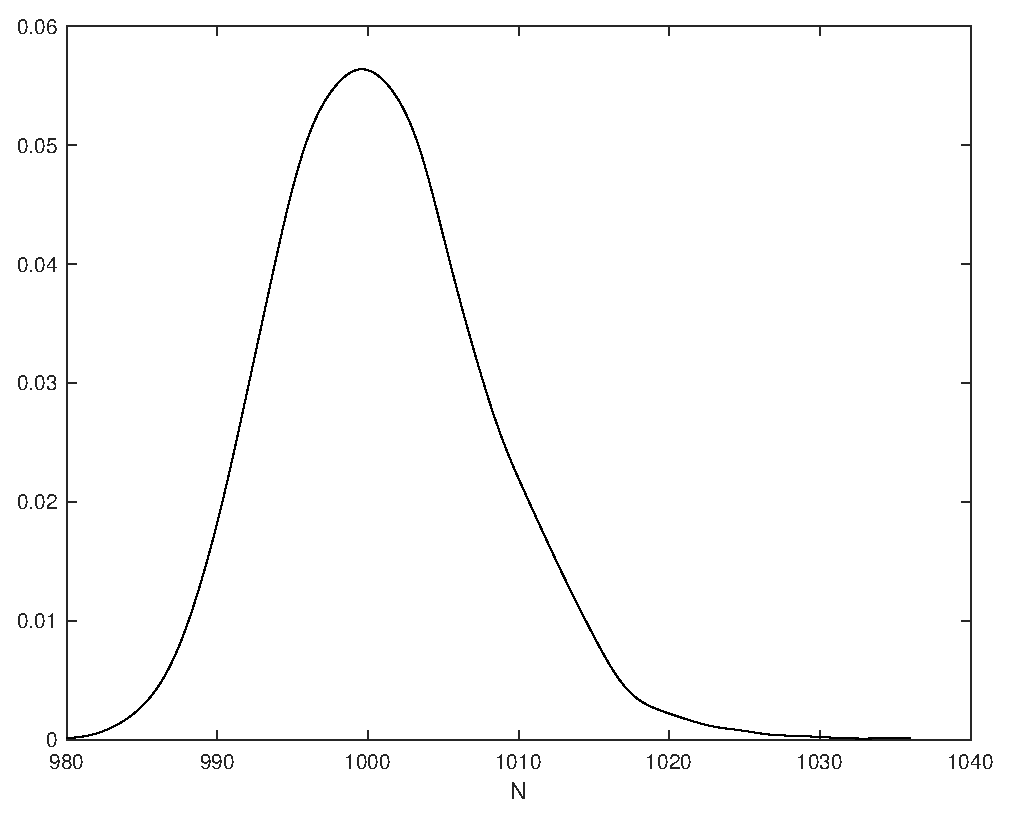
\includegraphics[width=12cm]{Image}
\caption{$P(N\mid \mathcal{N})$ against $N$, where $\mathcal{N}=$ \texttt{TestData} using the GSA}\label{fg:SimPDF}
\end{figure}
\begin{table}[H]
\centering
\begin{tabular}{|ccc|cc|}
\hline 0.05-Q &Median & 0.95-Q& Mean & Standard Deviation\\
\hline  990.0 & 1000.4 & 1013.3 & 1000.9 & 7.19\\
\hline
\end{tabular}
\caption{Diagnostics of $P(N\mid \mathcal{N})$, where $\mathcal{N}=$ \texttt{TestData} using the GSA}\label{tb:SimQUANT}
\end{table}
It can be seen that the method is indeed accurate, with the true value of $N$ centred well within the middle of the pdf. Not only this, but the variance is low, indicating a high confidence that $N$ is approximately 1000. This is a confident conclusion that this method is valid for the data in \texttt{ExtremeBB} with a high level of precision. Note that this code was run twice with different values of $M^{*}$. In both cases the sampled distribution was approximately the same, suggesting $M^{*}$ was chosen sufficiently large. This meets the requirements laid out in section \ref{sc:4.1}.

\section{Other Approaches}\label{sc:5}
In this section Silverman's alternative approaches to estimating $N$ are considered, and the reasons they weren't selected for the \texttt{ExtremeBB} dataset are presented. The section will end with a comparison of the methods using the original \texttt{HumanTrafficking} data. Note that these methods are described briefly, and that full descriptions can be found in the appropriate references.

\subsection{The Poisson Model}
Returning to equation \eqref{eq:Multinomial}, we can alternatively look for an approximation of the multinomial model. Silverman argues that one such approximation can be given by the multivariate Poisson distribution
\begin{equation}
P(\mathcal{N} \mid \bm{\lambda}, N)=\prod_{S\in \mathcal{P}(L)}\frac{(\lambda_{S})^{n_{S}}}{n_{S}!}\exp\left(-\lambda_{S}\right)
\end{equation}
where $\bm{\lambda}=\left(\lambda_{S}\right)_{S\in\mathcal{P}(L)}$ are shape parameters. The conditions when this approximation holds will not be discussed however it is important to note that this model is weaker than the multinomial as it does restrict the values the variables can take. The resultant model is a far simpler one where each $n_{S}\sim\text{Poisson}(\lambda_{S})$ although note that the $n_{S}$ are not necessarily independent as the $\lambda_{S}$ may depended on each other. Finding an estimate for $\lambda_{\emptyset}$ becomes sufficient to estimate $N$, as it provides an estimate for $n_{\emptyset}$.

\subsubsection*{Frequentest Approach}
Silverman further defined the model such that
\begin{equation}\label{eq:2}
\log(\lambda_{S})=\mu +\sum_{i\in S}\alpha_{i}+\sum_{\substack{i,j\in S\\i\neq j}}\beta_{ij}
\end{equation}
restricting this model further, since it assumes $n_{S}$ and $n_{T}$ are iid provided $S$ and $T$ share at least two elements. This is irrespective of the sizes of the sets $S$ and $T$, making this generally a weak model. To estimate $\lambda_{\emptyset}$ a maximum likelihood estimator (MLE) was proposed, however calculating a MLE for each interaction term $\beta_{ij}$ was thought to overfit the model. Hence for each combination of interaction terms, along with fixed effects $\alpha_{i}$ and $\mu$, the Akaike Information Criterion (AIC) was calculated and the minimum value was chosen. The AIC for a model $\mathcal{M}$ is defined as
\begin{equation}
\text{AIC}(\mathcal{M})=2k -2 \ell(\hat{\theta}^{\text{MLE}})
\end{equation}
where $k$ are the number of parameters in the model, $\ell$ denotes the log likelihood function and $\hat{\theta}^{\text{MLE}}\in \R^{k}$ denotes the MLE. It is a common choice for model selection, and an in depth analysis of it can be found in the paper \cite{AIC} by Bozdogan. By computing the MLE with the smallest AIC, this gives a final estimate for $\mu=\lambda_{\emptyset}$. 

There are some major drawbacks to this method. Firstly the number of models that the AIC has to be calculated for is of order $O((K^{2})!)$, making this unrealistic for a large number of lists. In Silverman's paper $K=6$ was computationally too big, and so this would have not been feasible for \texttt{ExtremeBB}. Other issues include the tight restrictions due to equation \eqref{eq:2}, and the possibility that the MLE does not exist, which may manifest itself as an infinite estimate for $n_{\emptyset}$ (see Chan \textit{et al}, \cite{Chan}). 

A method was proposed to solve the complexity problem by sequentially minimising the AIC; adding interaction terms $\beta_{ij}$ into the model one at a time, based on which lowered the AIC the most. This was iterated until a local AIC minimum was achieved, or if adding another parameter wasn't significant at some threshold $\tau$. In the paper \cite{Cormack} by Cormack, confidence intervals were developed for the final estimates. This method is a valid one, and if it were not for time limitations it would make for an interesting analysis.
\subsubsection*{The Bayesian-Threshold Approach}
Silverman proposed a new method under the same model called the Bayesian Threshold Approach. After defining uniform (improper) priors on $\mu$, $\alpha_{i}$ and Gaussian priors (mean 0 variance $1/\lambda$) on $\beta_{ij}$, the posterior under the Poisson model was calculated. The posterior mean of each $\beta_{ij}$ was then calculated,  and any that didn't pass a threshold value $\tau$ were removed from the model before the same analysis was repeated. This was run until equilibrium was achieved.

The major drawback to this method is when the following property occurs in the data used: $n_{\{i,j\}}=0$, and $n_{S}>0$ for where $i,j\in S$. In this scenario $\beta_{ij}=-\infty$ with probability one (as shown by Silverman), and hence any model this method concludes will be wrong, as it will predict $n_{S}=0$ for all sets $S$ that include $i,j$. This phenomenon was not frequent but did occur in the \texttt{ExtremeBB} data set, and hence this method was not chosen.

\subsection{The Graphical Method}
The final method used in Silverman's paper was a graphical method developed by Madigan and York in \cite{Madigan}, which uses every decomposable graph\footnote{A decomposable graph is one such that all of it's cycles of size greater than 3 have a chord; an edge that is not part of the cycle but connects two vertices within the cycle. } of dependencies between the lists $L$, and obtains posterior probabilities of the model and the population size $N$. It is proved by Castellví \textit{et al} in \cite{Chordal} that the number of labelled chordal planar graphs on $K$ vertices, that is to say the number of decomposable graphs, is asymptotically equal to  
\begin{equation}
\frac{g\gamma^{K}K!}{K^{5/2}}
\end{equation}
where $g>0$ is a constant and $\gamma \approx 11.9$. This can be seen to grow incredibly quickly in $K$; in particular when using the \texttt{ExtremeBB} dataset where $K=9$, there are 2192816760 models to check, making this method infeasible (see the online resource \cite{Graph}). 


\subsection{Comparison}
In this subsection we will compare the methods above to the GSA approach, using the small list dataset \texttt{HumanTrafficking}. Silverman has already applied the above methods to this data, and so it suffices to compute the quantiles of the posterior $P(N\mid\mathcal{N}=\texttt{HumanTrafficking})$ using the code \texttt{Gibbs-Sampler}. This algorithm was run multiples times with $M^{*}$ equalling 50 and 100, while setting the values $a$ and $b$ to 10 and 20 respectively and the number of iterates to 10000 with the first 5000 as a burn in period. The data is presented in Table \ref{tb:4}, along with the data published by Silverman in \cite{Silverman}.

\begin{table}[H]
\centering
\begin{tabular}{|cccccc|}
\hline Method & \multicolumn{5}{c|}{Estimates and confidence intervals}\\
& 0.025 & 0.1 & Point Estimate & 0.9 & 0.975\\ \cline{2-6}
Stepwise AIC ($\tau =0.001$) & 12.6 &13.1 &14.2 &15.4 &16.1\\
Stepwise AIC ($\tau =0.05$) & 9.9 &10.3 &11.3 &12.4 &13.1\\
\hline \hline  & \multicolumn{5}{c|}{Quantiles of posterior}\\
& 0.025 & 0.1 & 0.5 & 0.9 & 0.975\\ \cline{2-6}
Graphical Method & 10.4 & 11.3 & 23.0 & 29.6 & 33.3\\
Bayesian Threshold Approach ($\lambda= 1, \tau =2$)& 11.7 & 12.1 & 13.2 & 14.3 & 15.1\\
Bayesian Threshold Approach ($\lambda= 0.1, \tau =5$)& 12.0 & 12.5 & 13.5 & 14.6 & 15.3\\
Gibbs Sampler Algorithm & 10.8 & 11.2 & 12.1 & 13.2 & 13.8\\ \hline
\end{tabular}
\caption{Quantiles and point estimates (in thousands) for $N$ using \texttt{HumanTrafficking} data applied to Silverman's methods and the GSA}\label{tb:4}
\end{table}
We see that the GSA produces very close estimates to the other methods, confirming that it is a valid extension of those presented in the Silverman paper to large list data.

\section{Results and Conclusion}\label{sc:6}
In this section the results from applying the GSA to \texttt{ExtremeBB} are presented. A discussion surrounding the problems with these results and topics of further research are also included in a conclusion.

\subsection{Results}\label{sc:6.1}
The GSA was run on the data \texttt{ExtremeBB} over 3-month periods, spanning from 1st January 2018 to the 31st December 2020, using the code labelled \texttt{Gibbs-Sampler}. This provides 12 estimates of the value of $N$; the number of active online extremists in America. 

The values of $a$ and $b$ were set to 1 and 0.5 respectively to keep the probability model sparse. The GSA was iterated 10000 times, with the first 5000 being discarded as a burn in period. The values of $M^{*}$ changed for each time period, but the minimum value used was 200, with a variety tested to ensure the true posterior was achieved.

A Gaussian kernel was used to estimate the density $P(N\mid\mathcal{N})$ from the generated samples, from which the main quantiles, expectation and standard deviation were calculated. These quantities are tabulated below in Table \ref{tb:2} along with the total observed cases $n$. 

\begin{table}[H]
\centering
\begin{tabular}{|c|ccc|ccc|} \hline 
Date & $n$ & $\E[N\mid\mathcal{N}]$ & $\sqrt{\text{Var}[N\mid\mathcal{N}]}$&  5\%-Q&50\%-Q&95\%-Q\\ \hline
Jan - Mar 2018&12425 & 25675 & 1070 & 24034.1 & 25657.9 & 27456.5\\ 
Apr - Jun 2018 &11927 & 17832 & 544 & 16975.4 & 17802.0 & 18765.5\\ 
Jul - Sep 2018 &13174& 20291 & 682 & 19172.4 & 20305.5 & 21398.4\\ 
Oct - Dec 2018 &13293 & 26925 & 1107 & 25212.7 & 26898.0 & 28848.7\\ 
Jan - Mar 2019 &14888 & 33508 & 1438 & 31154.4 & 33559.3 & 35885.0\\ 
Apr - Jun 2019 &14691& 40127 & 1978 & 37016.7 & 40109.7 & 43562.4\\ 
Jul - Sep 2019 &14651& 24681 & 1036 & 23100.7 & 24628.7 & 26493.4\\ 
Oct - Dec 2019 &12973 & 29127 & 1402 & 27213.0 & 28889.2 & 31842.1\\ 
Jan - Mar 2020 &14724 & 31187 & 1354 & 29265.9 & 31083.7 & 33603.4\\ 
Apr - Jun 2020 &16916& 42935 & 1754 & 39957.5 & 42924.0 & 45853.6\\ 
Jul - Sep 2020 &17054& 25889 & 816 & 24640.7 & 25843.4 & 27248.7\\ 
Oct - Dec 2020 &16643 & 37561 & 1413 & 35354.5 & 37506.0 & 40067.3\\ \hline
\end{tabular}
\caption{Details of $P(N\mid\mathcal{N})$ using $\mathcal{N}=\texttt{ExtremeBB}$}\label{tb:2}
\end{table}
Notice the final estimates for $\E[N\mid\mathcal{N}]$ are approximately 1.5 to 3 times bigger than the number of observed cases $n$. The accuracy of each of these estimates are different, with the largest error being $\pm3\times 1978 \approx \pm6000$. 

To better portray this time sequential data, we will introduce the notion of a cubic spline. Given data $(x_{1},y_{1}),\hdots,(x_{n},y_{n})$ ordered by $x_{i}$, a cubic spline is a function $f(x)$ that satisfies the following properties. On the interval $[x_{i},x_{i+1}]$ it behaves as a cubic polynomial, and $f(x_{i})=y_{i}$. It also must have a continuous second derivative. It is a common method to interpolate data.

Cubic splines were fitted to the 0.05, 0.5 and 0.95 quantiles and plotted in Figure \ref{fg:1} below, along with $\E[N\mid\mathcal{N}]$ marked in black dots. The linear estimator for the mean values was also included in grey. This was computed using the code labelled \texttt{Data-Plot}.
\begin{figure}[H]
\centering
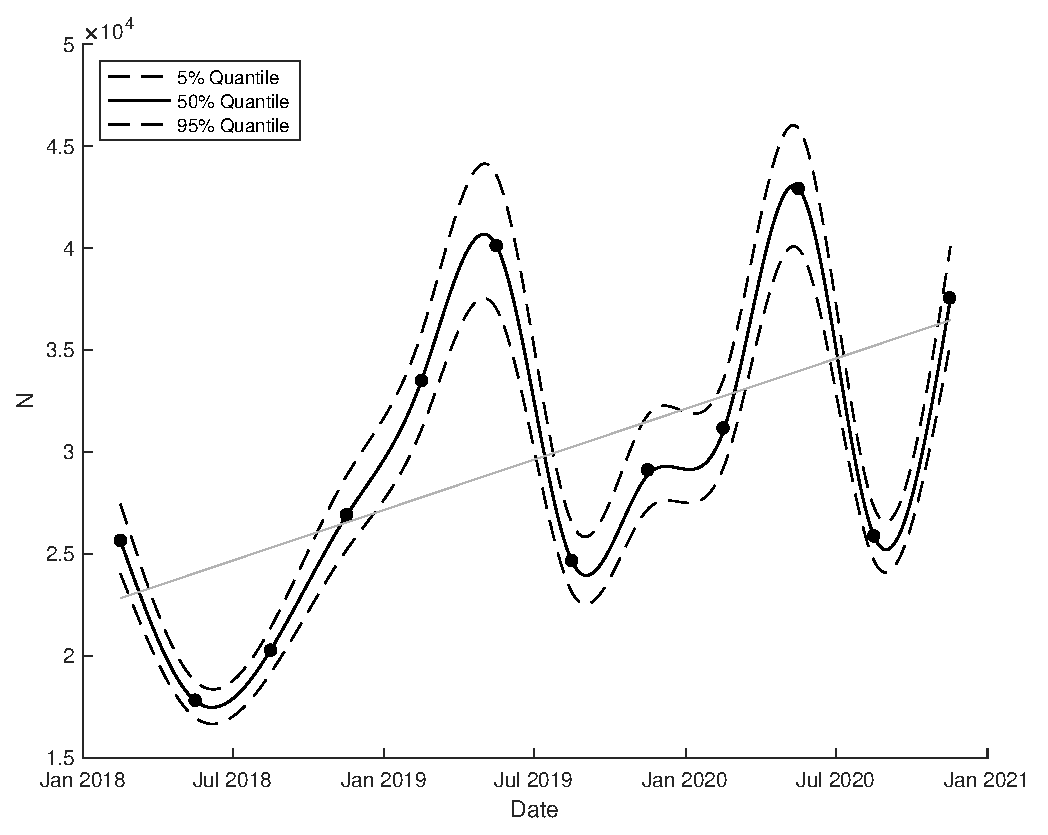
\includegraphics[width=12cm]{Results}
\caption{Time sequential estimates of $N$ using $\mathcal{N} = \texttt{ExtremeBB}$}\label{fg:1}
\end{figure}
The oscillatory nature of the estimates from January 2020 onwards make sense, with an increase in the value of $N$ coinciding with the start of the COVID-19 pandemic. This is likely due to the increased number of people at home with access to these forums after many were suspended from their jobs. The estimates drop around July 2020 as restrictions began to relax and those went back to work, and then increase as the second wave of COVID began in December 2020. This also coincides with the storming of the state capital in America on the 6th January 2021, providing evidence that this may have been influenced by an increase in online extremism.

Before January 2020, the data doesn't fit a particular trend but in general there is an increase in the number of online extremists. An unexpected result is the sharp increase in the estimates from June 2018 to June 2019, however this coincides with no relevant world events. An investigation into world affairs at the time might provide reasoning why this occurred.

The standard deviation of the estimates grows linearly with the size of estimates themselves, which can be observed from the data in Table \ref{tb:2}. This is a consistent observation when using the simulated data, where $N$ was relatively small, and the standard deviation was also consistently small. This suggests that should a confident estimate be given, then this method performs better when the inherent population is smaller.

The relation between the estimates $N$ and observed cases $n$ is now investigated. Although $n$ gives no information about the true value of $N$, it might gives some indication as to how $N$ has changed over time. A cubic spline was also fitted to $n$ before being scaled and translated such that it had the same empirical mean and standard deviation as that of the 0.5\% quantile data. These two curves are plotted below in Figure \ref{fg:2}.

\begin{figure}[H]
\centering
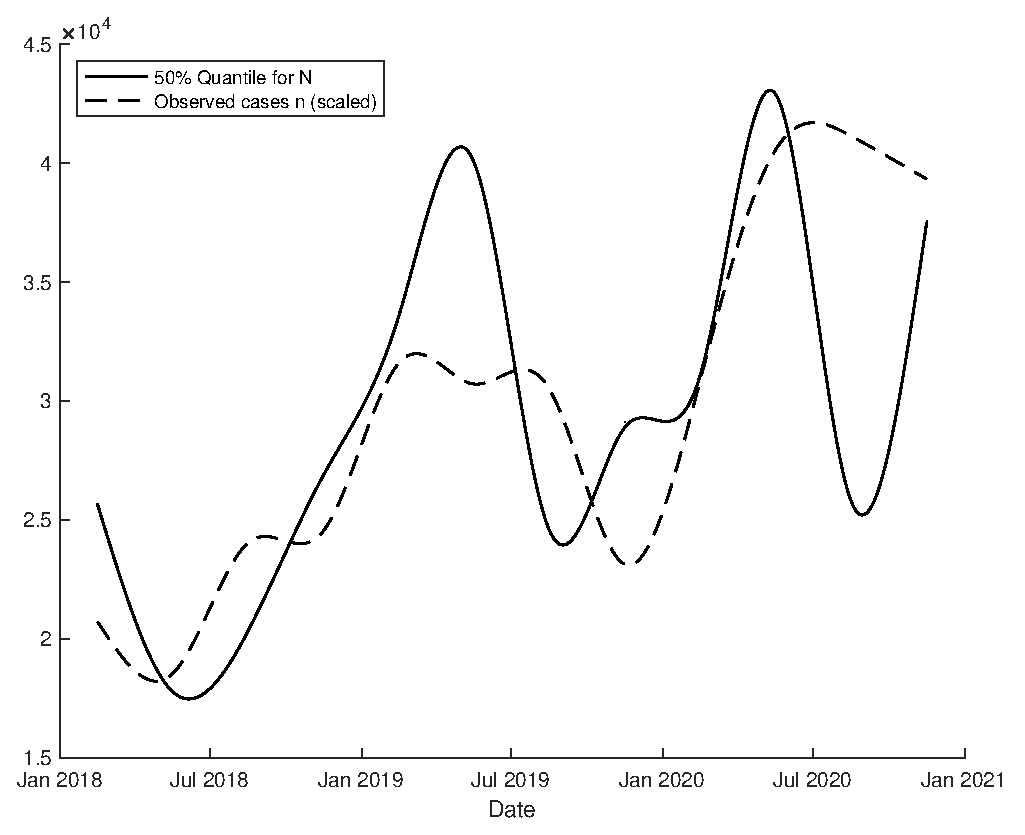
\includegraphics[width=12cm]{Results2}
\caption{Comparison of 50\% quantile for $P(N\mid\mathcal{N})$ to observed cases $n$, using $\mathcal{N}=\texttt{ExtremeBB}$}\label{fg:2}
\end{figure}
Both curves exhibit an increase in the number of online extremists, however there are moments where these curves differ. The number of observed cases $n$ is disproportionately small in June 2019, and disproportionately large in September 2020. This highlights the importance of cross forum analysis; that by just comparing the number of observed cases without overlaps it appears that recently cases have been decreasing, whereas this essay concludes there's been a large increase. This is not to say analysing $n$ is not useful over a large time period since it's curve approximately matches $N$, however for a more detailed analysis it fails.

\subsection{Conclusion}
Although the increase in active online extremists based in America is a valid conclusion, it may be due to other factors. In the last section of this essay, possible improvements are discussed, as well as further research.

Analysing 9 forums is likely to give biased results, and the analysis should include a larger pool of online extremism. This is a difficult task as it's believed the vast majority of extremist hate is shared privately and so is difficult to source, but it is certainly a topic of great interest. The sharp increase in the estimates from June 2018 to June 2019 is interesting, and an analysis of world events at the time might provide a clear explanation, however this may also be a feature of the bias in these forums. This analysis uses only American data, and comparing global data would produce interesting results.

No analysis of the comments posted on these forums was taken into account, with some users possibly being 'more radical' than others. The computer laboratory at Cambridge has built a metric to define how 'toxic' a comment is, and incorporating this into the classification criterion may yield different results. The metric can be found in the paper \cite{ExtremeBB}.

With respect to the method itself, although it copes successfully with data that fall into many lists, it struggles when the size of the observed cases $n$ increases, as this is directly related to the number of $\bm{z}$ variables in the model. Therefore devising a method that grows with a smaller number of variables would be useful, especially as these datasets increase in size. A further study into the quantiles of the posterior distributions may help improve the certainty of the results, or motivate a new approach should the standard deviations grow to large.

The cross forum analysis will always be difficult to classify, although the increase in data collection will hopefully limit this, through methods such as more accurate posting distribution comparison, or by comparing attributes, such as the geolocation of where posts are made.

An in depth analysis of the stepwise AIC model applied to this online data may help to give a better understanding of the value of $N$. Provided the results are consistent to the ones in section \ref{sc:6.1}, then this provides a stronger conclusion than the one in this essay.\\ \\


Online extremism's influence on the modern world is a largely misunderstood topic. The lack of regulation on social media has allowed it to grow both privately and publicly, but understanding how it has impacted world events such as the storming of the state capital is not yet known. Producing simple estimates like the ones presented in this essay, and combining results from different sources, may help to provide evidence that the two are mutually linked. Censoring online extremism (hate speech) is a highly ethical debate, as it infringes the right to freedom of opinion and expression. Until concrete evidence is presented for the impact of online extremism, hate speech will continue to be a part of the American society. Because of this, it is a hugely interesting topic for research.

\printbibliography
\end{document}
